\documentclass{article}
\usepackage{tikz}
\usepackage{pgfplots}
\pgfplotsset{compat=1.16}

\begin{document}
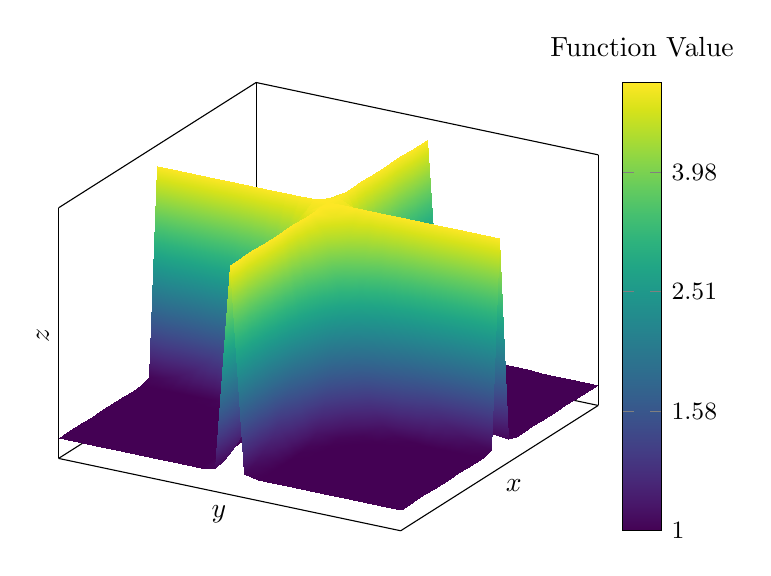
\begin{tikzpicture}
    \begin{axis}[
        view={120}{30},   % set view angle
        xlabel={$x$},
        ylabel={$y$},
        zlabel={$z$},
        ticks=none,
        domain=-1:1,
        colormap/viridis,
        colorbar,
        colorbar style={
            title={Function Value},
            ylabel style={font=\small},
            yticklabel style={font=\small},
            yticklabel={\pgfmathparse{10^\tick}\pgfmathprintnumber{\pgfmathresult}}
        }
    ]
    \addplot3[surf,shader=interp] {.75/exp((x*5)^2*(y*5)^2)};
    \end{axis}
\end{tikzpicture}
\end{document}